\chapter{Анализ масштабируемости, параллельной эффективности и ускорения параллельной ВС}
			%	ОБЩЕЕ ПРАВИЛО ДЛЯ ВТОРОЙ ГЛАВЫ: НЕ ПЛАНРИРОВАТЬ ЧТО_ТО НОВОЕ И ОЧЕНЬ ХОРОШЕЕ ЧЕГТО НЕТ, А ПОДКРЕЛЯТЬ И УИСИЛВАТЬ ТО, ЧТО РЕАЛЬНО ЕСТЬ.
			%	ЕСЛИ У НАС СЛАСБОСТЬ В ОБЛАСТИ АНАЛИЗА КОММ СТРУКТУРЫ - НУ И ЛАДНО, И ПУСТЬ ОНА БУДЕТ. ГОВОРИТЬ БОЛЬШЕ О МАСШТАБИРУЕМОСТИ. А КОРММ СТРУКТУРУ АНАЛИЗИРПОВАТЬ ЧЕРЕЗ ПЕРЕСЫЛКИ ЧАСТИЦ
			%	НАША ИДЕЯ не ПОДМЕНЯТЬ СОБОЙ ДИАГНОСТИКУ АРХИТЕКТУРЫ, а мерять И ОПРЕДЕЛЯТЬ ВСЕ ЧЕРЕЗ ИЗМЕРЕНИЯ ВРЕМЕН ПО PIC
				В четвертой главе предложена методика интегральной оценки тестируемой ВС с помощью измерения масштабируемости с расчетах по методу частиц в ячейках и определения на основе измерений возрастания потока данных в коммуникационной сети ВС.
%				На основе данных о пересылке модельных частиц измерена производительность коммуникационной сети ВС, при этом важно отметить преимущества использованного метода измерений: пересылка данных имеет высокую степень нерегулярности, а также большой объем, что означает проведение тестирования на большой нагрузке, и возможность широкого применения полученных таким образом данных.
%				Также предложена и апробирована методика определения фактически соседних (с точки зрения MPI) узлов ВС.  

            Основной вопрос четвертой главы заключается в следующем: что можно сказать о вычислительной системе и о перспективах ее использования для решения различных задач на основании тестирования с помощью метода частиц в ячейках. 
            
            В частности, в данной главе определяется новое понятие эффективного коммуникационного размера ВС, имеющего
             смысл максимального количества процесоров, которое может быть в рамках данной ВС эффективно использовано для решения одной задачи.  
							
			\section{Определение понятий эффективности, масштабируемости и ускорения}
			%\textbf{Степаненко, книжка"высокопроизводительные вычисления", учебник Воеводина}
			
			Выписано определение эффективности параллельной реализации программ, сильной и слабой масштабируемости, ускорения при распараллеливании.
			
			В частности, ускорение параллельного алгоритма для $N$ процессоров, определяется как:
			$$
			S_N = \frac{T_1(n)}{T_N(n)}
			$$  
			здесь $T_1$ - время исполнения алгоритма на одном процессоре, $T_N$ - на $N$ процессорах, величина $n$ характеризует вычислительную сложность решаемой задачи, для определения ускорения существенно, что задачи, решаемые на 1 и на $N$ процессорах имеют одинаковую сложность.
			Далее, эффективность распараллеливания вычисляется как
			$$
			\eta_N = \frac{1}{N}\frac{T_1(n)}{T_N(n)}
			$$  
			эта величина иногда называется эффективностью в сильном смысле (англ. strong efficiency). Кроме того, часто используется эффективность в слабом смысле (англ. weak efficiency):
			\begin{equation}
			\label{weak_eff}
			\eta^{weak}_N = \frac{T_1(1)}{T_N(N)}
			\end{equation}
			здесь, в отличие от определения ускорения, задачи, решаемые на одном и на $N$ процессорах, имеют различную сложность, т.е. при увеличении количества процессоров в $N$ раз сложность задачи такжэе увеличивается в $N$ раз, и таким образом определяемая эффективность будет 100 \% в том случае, если время вычислений не возрастает при увеличении сложности задачи пропорциональном увеличению количества процессоров.   
			
			Приведены различные используемые варианты этих определений, перечислены факторы, влияющие на  значения этих величин для конкретной ВС, а именно скорость обмена данными и структура коммуникационной сети ВВС, алгоритмы реализации MPI-процедур, в особенности коллективных, настройки коммуникационной системы (таймауты, размер системных буферов, и др.).
			%\textbf{написать формулы} 
			%\textbf{привести формулы из статьи в СибЖВМ}
			Для последующего анализа измереннного времени работы метода частиц в ячейках на параллельной ВС, и для прояснения зависимости этого времени от параметров расчета можно привести следующую схематическую формулу для длительности одного временного шага, аналогично статье (Вшивков В.А. и др., СибЖВМ, 2003):
			
			\begin{equation}
			\label{PIC-timestep}
			T=T_{F} \left ( \frac{N_x N_y N_z }{P_E}\right )+ T_{F,S}\left (N_y N_z\right ) + T_P\left(\frac{N_p}{P_E\times P_L}\right) +T_{P,S}\left (\frac{N_p*T_p}{P_E\times P_L}\right)
		\end{equation}
			 
		здесь $T_{F}$ - время вычисления электромагнитного поля, $N_x, N_y, N_z$ - размер расчетной сетки соответственно, по координатам $X$ $Y$ и $Z$, $P_E$ - количество процессоров для эйлеровой декомпозиции, т.е. для разделения расчетной области на подобласти, $T_{F,S}$ - время, затрачиваемое на персылку граничных значений полей и токов между подобластями, которое зависит только от $N_y$ и $N_z$ в силу того что на данный момент используется одномерная декомпозиция,  $T_P$ - время расчета движения частиц, $P_L$ - количество процессов (или потоков) для лагранжевой декомпозиции, т.е. для дополнительного разделения частиц подобласти на группы, вычисляемые на отдельных ядрах.
		
		\section{Формулы для анализа данных о масштабируемости}
		
			\begin{equation}
			\label{weak_eff}
			\eta^{weak}_N = \frac{T^1(1)}{T^N(N)}
			\end{equation}
			здесь $T^K(N)$ обозначает время счета задачи с характерной размерностью $K$ при использовании $N$ процессоров.
			это время состоит из двух основных частей:
			\begin{itemize}
				\item собственно времени счета $T^K_{P}(N)$;
				\item времени коммуникаций $T^K_C(N)$;
			\end{itemize}
			Таким образом,
			\begin{equation}
			\label{weak_eff_detailed}
			\eta^{weak}_N = \frac{T^1(1)}{T^N_{P}(N)+T^N_C(N)}
			\end{equation}
			при выполнении вычислений одновременно на однотипных процессорах
			можно считать, что $T^1(1) = T^N_C(N)$, таким образом формула
			\ref{weak_eff_detailed} приводится к виду:
			\begin{equation}
			\label{weak_eff_detailed-time}
			\eta^{weak}_N = \frac{1}{1+ \frac{T^N_{C}(N)}{T^1(1)}}.
			\end{equation}
			Это означает, что при известном времени расчета задачи на одном процессоре можно восстановить время коммуникаций по эффективности в слабом смысле:
			\begin{equation}
			\label{comm_time_from_efficiency}
			T^N_{C}(N) = T^1(1) \left(\frac{1}{\eta^{weak}_N} - 1\right)
			\end{equation}
			далее время коммуникаций может быть источником для вычисления производительности коммуникационной сети при известном объеме пересылок.
			
			
			
		
		
		
	
	    \section{Вычисление характеристик коммуникационного оборудования ВС на основе измеренной масштабируемости метода частиц в ячейках}
	    
	    
	    
	    В этом разделе показаны измереннные характеристики масштабируемости параллельной программы, реализующей методж частиц в ячейках на кластере НГУ. Для того, чтобы исключить вопрос о неточности измерений коомуникационного времени внутри программы, в этом разделе измерения проводились с помощью Intel Trace Analyzer \& Collector.
	    
\begin{figure}[h]
\begin{center}
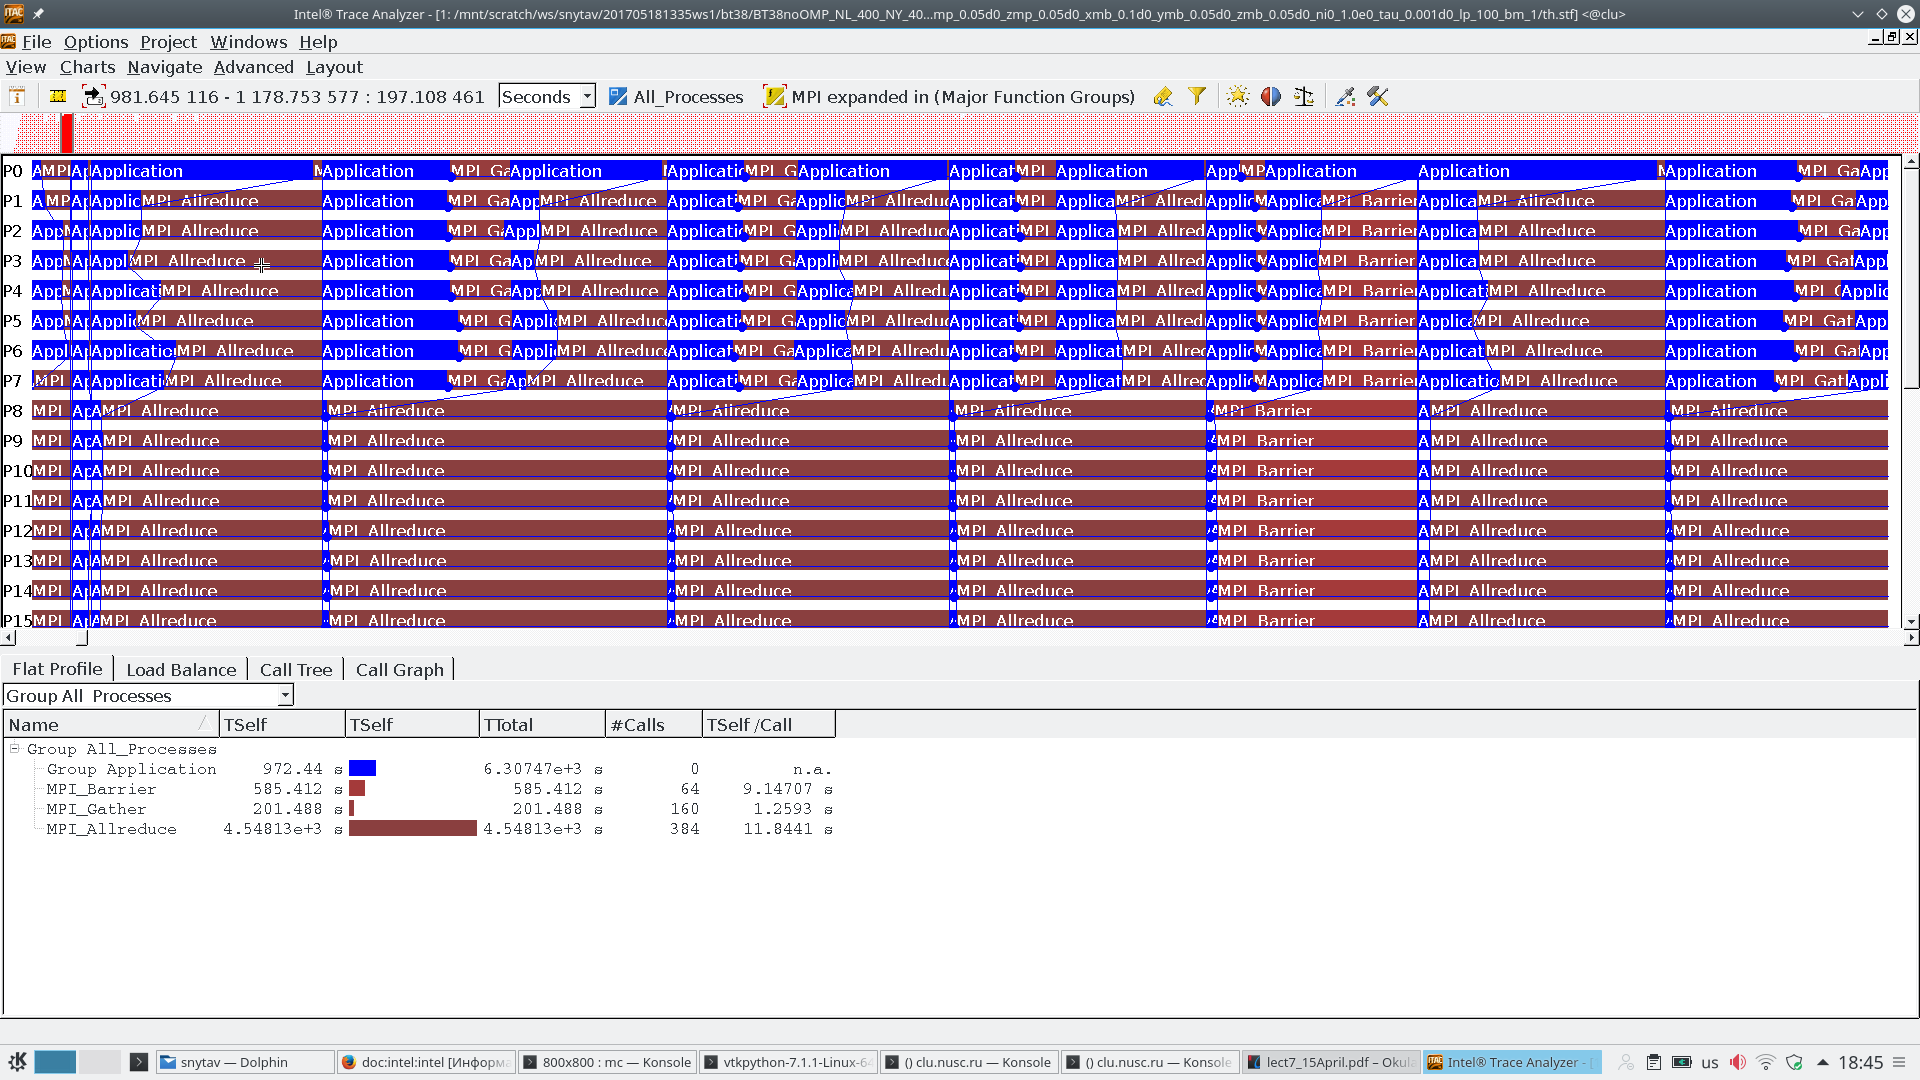
\includegraphics[height=5cm,keepaspectratio]{images/scalingNSU-img17.png}
\caption{
Результат профилировки программы с помощью Intel Trace Analyzer \& Collector на кластере НГУ. Горизонтальные линии(трассы) означают отдельные параллельные процессы, тонкие линии между трассами – межпроцессорные коммуникации, номера процессов показаны слева (от 0 до 15, всего 32 процесса). Красный цвет трассы означает пересылки, синий-счет. Показан отдельный интервал расчета на сетке 800×800×20, на 32 процессорах.
}
\label{scale8}
\end{center} 
\end{figure}
	   
	   
	    Результат показан на рисунках 
\begin{figure}[h]
	\begin{center}
		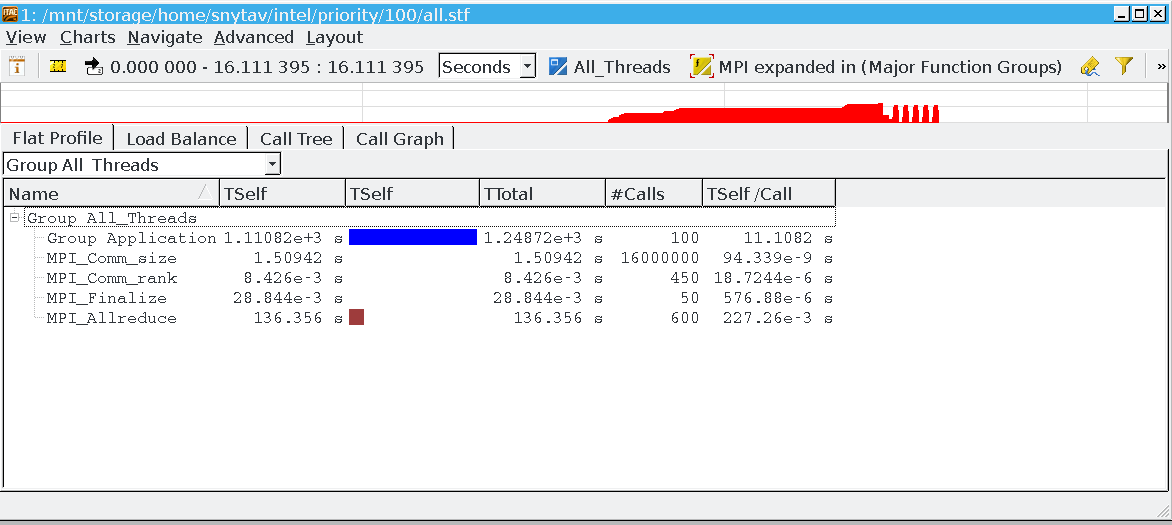
\includegraphics[height=5cm,keepaspectratio]{images/scalingNSU-img18.png}
		\caption{
		 Время выполнения коммуникационных операций (названия операций даны на рисунке, время показано красным цветов в графе TSelf) в программе в сравнении с временем вычислений (Group Application, синий цвет в графе TSelf). Расчет на сетке 1000×1000×4 узла,10 временных шагов, 100 частиц в ячейке,  100 процессорных ядер. Результат профилировки программы с помощью Intel Trace Analyzer \& Collector на кластере НГУ.
		}
		\label{scale9}
	\end{center} 
\end{figure}	    
	   
	   
\begin{figure}[h]
	\begin{center}
		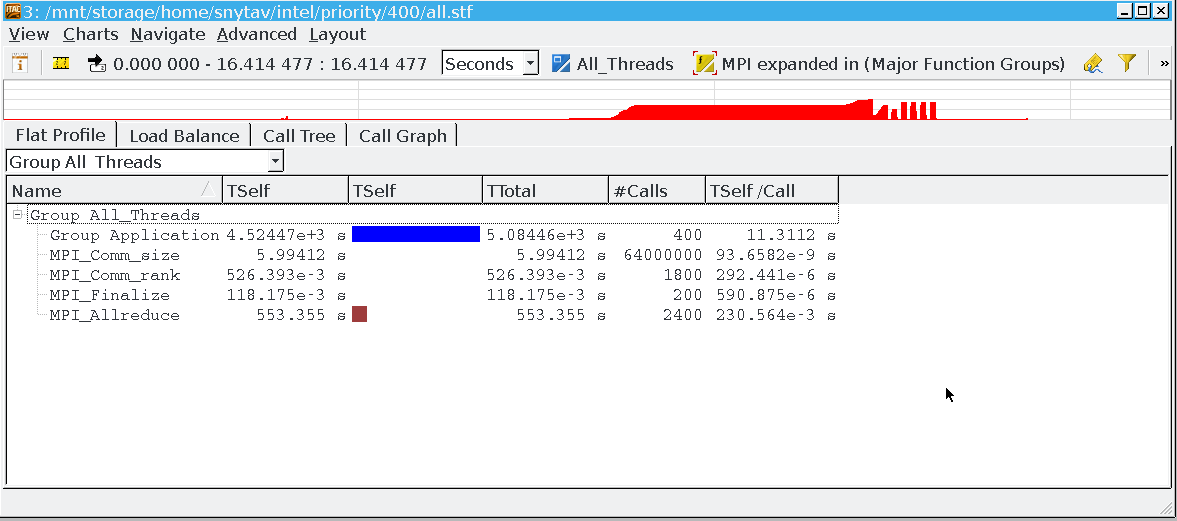
\includegraphics[height=5cm,keepaspectratio]{images/scalingNSU-img20.png}
		\caption{
			Время выполнения коммуникационных операций (названия операций даны на рисунке, время показано красным цветов в графе TSelf) в программе в сравнении с временем вычислений (Group Application, синий цвет в графе TSelf). Расчет на сетке $1000  \times 1000 \times 4$ узла, 200 частиц в ячейке, 400 процессорных ядер. Результат профилировки программы с помощью Intel Trace Analyzer\&Collector на кластере НГУ.
		}
		\label{scale9a}
	\end{center} 
\end{figure}	    
	    
	    
	   

\begin{figure}[h]
	\begin{center}
		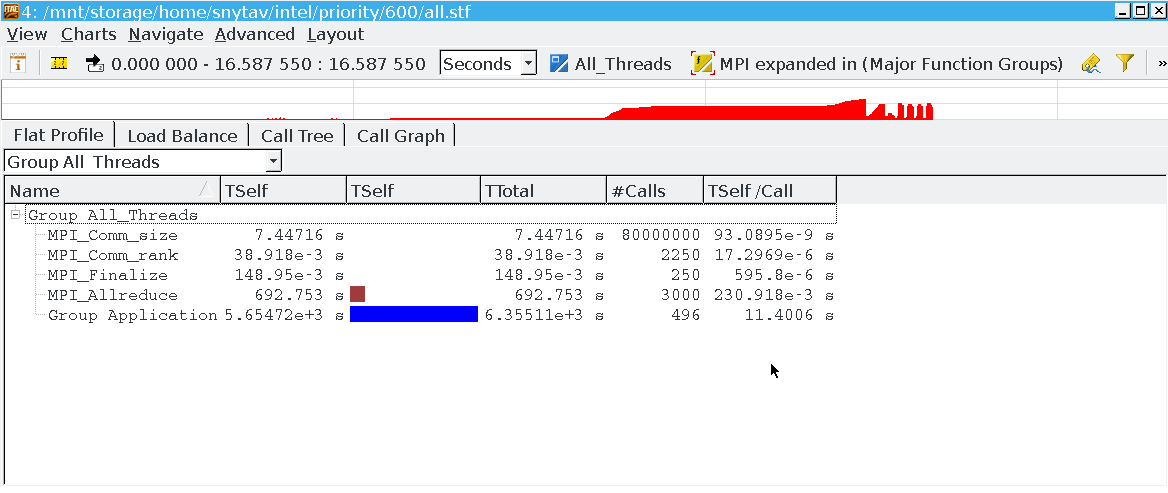
\includegraphics[height=5cm,keepaspectratio]{images/scalingNSU-img21.png}
		\caption{
		Время выполнения коммуникационных операций (названия операций даны на рисунке, время показано красным цветов в графе TSelf) в программе в сравнении с временем вычислений (Group Application, синий цвет в графе TSelf). Расчет на сетке 1000×1000×4 узла, 600 частиц в ячейке, 600 процессорных ядер. Результат профилировки программы с помощью Intel Trace Analyzer \&Collector на кластере НГУ
		}
		\label{scale10}
	\end{center} 
\end{figure}
	 
Сводя полученные результаты измерения времени воедино, получаем таблицу \ref{scalingNSUtab}.
   
	    
	   
\begin{table}[ht]
	\begin{center}
		\caption{Время вычислений и время комуникаций в зависимости от числа  процессов.}
		\begin{tabular}{|c|c|c|c|c|c|}
\hline			
Число        & Число    & Время вычислений               & Время        & Объем        &  производительность \\
процессорных & частиц   & (суммарное по всем процессам), & коммуникаций,& пересылаемых &  коммуникационной\\
ядер         & в ячейке & в секундах                     & в секундах   & данных, ГБ   &  сети, $W_A$,ГБ,сек.\\ \hline
 100         &  100     &  1248                          &  136         & 0.089        &  0.00065   \\\hline
 200         &  200     &  2543                          &  278         & 0.089        &  0.00032   \\\hline
 400         &  400     &  5084                          &  553         & 0.089        &  0.00016   \\\hline
 600         &  600     &  6335                          &  692.7       & 0.089        &  0.00012   \\\hline
 		\end{tabular}
 		\label{scalingNSUtab}
 	\end{center}
 \end{table}    
	    
	   
\begin{figure}[h]
	
	
	\begin{center}
		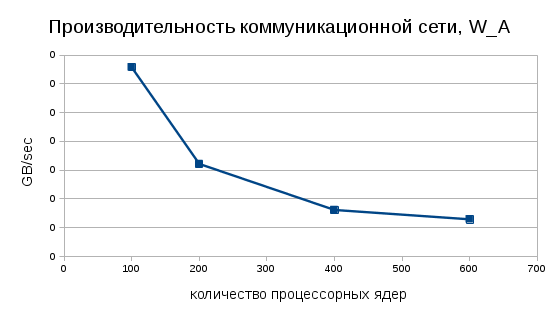
\includegraphics[height=5cm,keepaspectratio]{images/scaleNSU_W_A.png}
		\caption{
		 Производительность коммуникационной сети для коллективных пересылок (величина W_A, формула \ref{Net_performance_collective}). Расчет на сетке $1000 \times 1000 \times 4$ узла. Измерение времени проведено с помощью Intel Trace Analyzer\& Collector на кластере НГУ.
		}
		\label{scale_W_A}
	\end{center} 
\end{figure}
     Здесь мы подходим решению основного вопроса главы 4, и одного из основных для всей диссертационной работы в целом - а именно вопроса о том, что расчет по методу частиц может прояснить в отношении ВС на которой он выполнялся. Для этого определим новую характеристику ВС:
     
     \underline{\textbf{Определение}}: Эффективный коммуникационный размер ВС - максимального количества процесоров, которое может быть в рамках данной ВС эффективно использовано для решения одной задачи.  
     
     
     
     Осорбую важность представляет вопрос о коммуникационной связности ВС, т.е о том, до какой степени она способна функционировать как целое для решения одной большой задачи. Для решения этого вопроса предлагается перейти от масштабируемости как характеристики программы для решения задачи к анализу графика измнения производительности коммуникационной сети, полученного на основе данных о масштабируемости, т.е графика \ref{scale_W_A}. Далее необходимо тем или иным способом выделить на этом графике участок с большими значениями производительности коммуникационной сети.
     Один из возможных вариантов показан на графике \ref{scale_W_A_exp}, где показана аппроксимация этой зависимости гауссоидой. Далее ширина этой кривой (126) суммируется с начальной точкой (100), и полученное значение (226) и является эффективным коммуникационным размером данной ВС. Т.е. в данном чслучае эффективный коммуникационный размер - это количесво процессров, для которого производительность коммуникационной сети падает не более чем в $e$ раз по сравнению с максимальной.
     
     
\begin{figure}[h]
	
	
	\begin{center}
		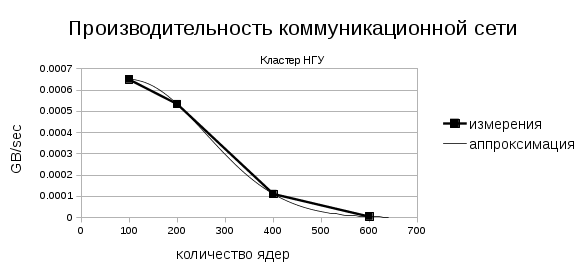
\includegraphics[height=5cm,keepaspectratio]{images/scaleNSU_exp_fit.png}
		\caption{
			Производительность коммуникационной сети для коллективных пересылок (величина W_A, формула \ref{Net_performance_collective}) - синие точки, и ее аппроксимация гауссовой кривой. 
		}
		\label{scale_W_A_exp}
	\end{center} 
\end{figure}     
\clearpage	    
	    
	 

		
		
		\section{Анализ масштабируемости как интегральной характеристики ВС.}
		
		Во втором разделе приведены фактически измеренные на различных высокопроизводительных ВС графики масштабируемости и параллельной эффективности и на основе этих данных проведен анализ коммуникационной сети данных ВС, в частности, для МВС-100К, рис. \ref{eff2}. 
		
		\begin{figure}[h]
			\begin{center}
				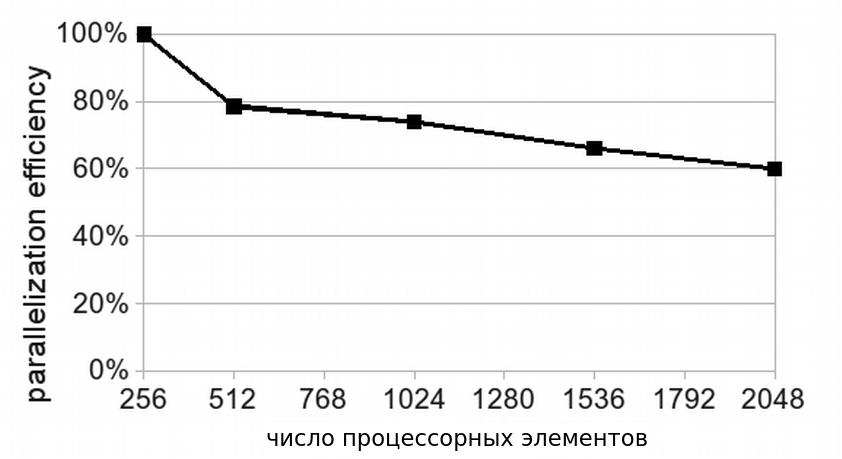
\includegraphics[height=5cm,keepaspectratio]{images/eff_weak_JSCC.png}
				\caption{
					Эффективность распараллеливания в слабом смысле, для МВС-100К, МСЦ РАН.
				}
				\label{eff2}
			\end{center} 
		\end{figure}
		
		Возможность проведения анализа коммуникационной сети с помщью расчетов по методу частиц в ячейках основана на известной информации о количестве пересылаемых данных и о виртуальной топологии, используемой в программе.
		
		Размер данных, перемещаемых между двумя соседними MPI-процессами равен $144 \times N_y N_z  $ байт. При этом в идеальном случае, когда соседние MPI-процессы находятся на соседних узлах, коммуникации происходят только между соседними узлами, и поток данных в системе в целом не возрастает с ростом количества используемых в расчете узлов.
		
		В частности, в расчете показанном на рис. \ref{eff2} использована эйлерова декомпозиция. Это означает, что используются только парные пересылки MPI, коллективные пересылки не используются, и поток данных через коммуникационную систему ВС в целом возрастать не должен. Если, тем не менее, он возрастает, что видно на рис. \ref{eff2} в виде снижения эффективности распараллеливания, то это может (при отсутствии коллективных операций), означать, что соседние с точки зрения MPI процессы находятся на физически удаленных друг от друга узлах параллельной ВС.
		
		Обозначая $k_{||}$ зависимость коэффициента при времени пересылок граничных условий от количества процессоров в формуле \ref{PIC-timestep}, так что 
		\begin{equation}
		T_{F,S} = k_{||} (P_E) \frac{N_y N_z}{P_E}
		\end{equation} 
		и подставляя формулу \ref{PIC-timestep} d \ref{weak_eff}, рассматривая только лишь время расчета и пересылок электромагнитного поля, можно получить 
		\begin{equation}
		k_{||} (P_E) = \frac{1}{\eta^{weak}(P_E)} - 1
		\end{equation}	  
		Таким образом величина $k_{||} (P_E)$  - \textbf{степень нелинейности} коммуникационной структуры параллельной ВС. Фактически она представляет собой отклонение от линейной функции для зависимости времени пересылок от количества процессоров. Он показывает предел возрастания потока данных через коммуникационную структуру ВС при увеличении количества процессоров, используемых в расчете. Эта величина характеризует, в какой степени при передаче информации между соседними процессами в MPI используются узлы параллельной ВС, не являющиеся ближайшими соседями. В силу того, что на значение эффективности оказывает влияние не только свойства оборудования, но и особенност реализации MPI, возникает необходимость разделить эти факторы. Это достигается с помощью привязки процессорв к узлам. 
		
		В итоге, такимобразом определенная  величина $k_{||} $ может быть использована как характеристика параллельной ВС, показывающая реально достижимую с помощью данной ВС эффективность и масштабируемость.
		
		Что касается масштабируемости как интегральной характеристики ВС,то хорошая масштабируемость на коллективных, очевидно нелинейных коммуникациях является важным показателем связности (сохранения произв. сети при увеличении ее размера) ВС и пригодности ее к решению одной большой задачи.
		
		\subsection{Измерение продолжительности параллельных коммуникаций и анализ характеристик и топологии коммуникационного оборудования}
		Здесь описано решение задачи об определении соседства процессов по реальным узлам. Это исключительно важно для производительности реальных задач, чтобы виртуально близкие (т.е. по номеру MPI-процесса) процессы исполнялись бы на соседних узлах многопроцессорной ВС. Для этого проводится обмен сообщениями между узлами, выделенными 
		для исполнения программы по топологии полного графа, и проводится анализ времени прохождения сообщений, рис. \ref{poly_all2all}.  
		
		Следует отметить, что такого этапа, с обменом сообщениями между всеми процессами в рамках метода частиц нет, поэтому, такой анализ проводится предварительно, перед запуском основной части программы.

		
		\begin{figure}[htb]
			\begin{center}
				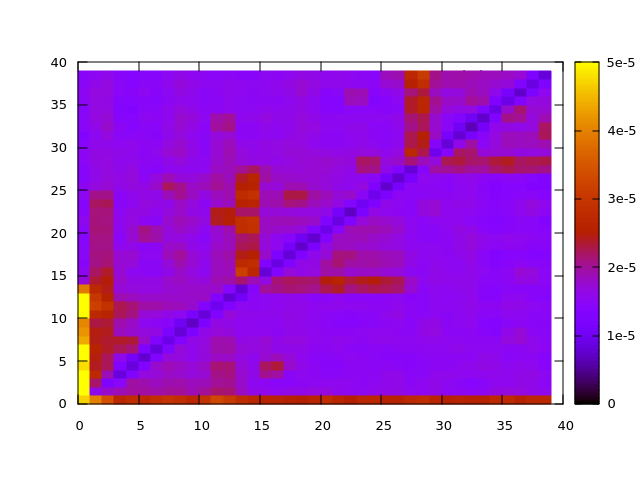
\includegraphics[height=7cm,keepaspectratio]{images/polytech_all_to_all.png}
			\end{center}
			\caption{Время пересылок для 40 MPI-процессов, расположенных на 10 узлах по 4 процесса, кластер «Политехник», СПбПУ. По осям X и Y отложены номера процессов, цветовая шкала показывает время пересылок в секундах.}
			\label{poly_all2all}
		\end{figure} 
		Узлы с минимальным временем считаются близкими, т.е. выясняется фактическая топология ВС. Это сопоставляется с известной информацией о размещении процессов по узлам.	Для повышения производительности приложения в дальнейшем целесообразно передвинуть соседние процессы на те узлы, где по факту меньше задержка по коммуникациям.
		
		%	\textbf{картинку из стьатьи все-со-всеми, (с Политеха)}. 
		%	1.измерение всех видов MPI-коммуникаций, сравнение одного с другим (Send, Isend, Bsend) - и увязатиь это с алгоритмом
		%	2. варьирование размера сообщений и пр. параметров
		
	%	\textbf{материал статьи НГУ ИТ  с более аакуратным анализом}
        \section{Оценки параллельной масштабируемости на основе измерений времени прохождения сообщений}
        
        Основные вопросы заключаются в следующем:
        \begin{itemize} 
        \item Что, если группа процессов, которые должны осуществлять коллективные пересылки, окажется размещенной на узлах суперЭВМ, расположенных физически далеко друг от друга, так что время выполнения этих пересылок будет велико?
        \item Как можно избежать такой ситуации, как объединять в группы для коллективных пересылок близко расположенные процессы, при том что MPI (или система очередей) размещает процессы на узлах фактически случайным образом? 
        \item Как можно заранее оценить трудоемкость коммуникационных операций и выработать оптимальную схему размещения процессов? 
        \item На основании чего можно принимать решение о перемещении процессов с одного узла на другой, или о перенумерации процессов?
        \end{itemize} 
        В некоторых случаях эти вопросы решаются специально созданными внешними инструментами [10, 11], но для рассматриваемой в данной работе программы целесообразным является иметь собственные средства для решения проблемы неудачного размещения на узлах.
        Для того, чтобы частично ответить на эти вопросы, были проведены вычислительные эксперименты на нескольких суперЭВМ с измерением производительности различных коммуникационных операций, построены оценки трудоемкости этих операций и предложен метод выделения групп близко расположенных процессов. Создать правильное представление о реальной длительности коммуникаций между процессами в программе важно также для того, чтобы решить вопрос о целесообразности использования динамической балансировки и для выбора конкретного ее варианта [12-14], и о применении форм-факторов высокого порядка [15-16] в методе частиц в ячейках [17,18, 19]. 
        
        \textbf{Краткое описание проведенных тестов}
        
        Задавались следующие основные параметры и числовые характеристики тестовых расчетов:
         \begin{itemize} 
        \item $N_X, N_Y, N_Z$  - размер сетки по каждому из измерений ($N_X$, $N_Y$ – от 100 до 500, $N_Z$ = 20)
        \item $P_{ALL}$  - общее количество процессорных ядер (до 1000)
        \item $P_{SUB}$  - число подобластей (до 20)
         \end{itemize} 
        Измерялись кроме физических величин, следующие времена (с помощью Intel Trace Analyzer \&Collector, https://software.intel.com/en-us/intel-trace-analyzer):
         \begin{itemize} 
        \item $T$ – длительность тестового расчета (50 временных шагов), сек.
       \item  $t$  - длительность временного шага, сек.
        \item $T_{MPI\_All}$ - длительность операции MPI\_Allreduce (суммирование токов по всей области), сек.
        \item $T_{MPI\_Send}$ - длительность операции MPI\_Sendrecv (обмен граничными значениями), сек.
        \end{itemize}
        
        
        
        Расчеты проводились на следующих суперЭВМ:
        \begin{itemize}
        \item Кластер НГУ. Из различных имеющихся типов узлов использовались только узлы  HP BL2x220c G6, каждый из которых содержит две материнские платы, на каждой из которых: два 4-ядерных процессора Intel Xeon E5540 с тактовой частотой 2530 МГц и 16 ГБ ОЗУ.
        \item Кластер СПбПУ «Политехник». Использовались узлы с двумя 28-ядерными процессорами  Intel®Xeon® E5-2600 v3.
        \item Кластер «Ломоносов» в НИВЦ МГУ. Использовались узлы основного раздела, содержащие 2 4-ядерных процессора Intel Xeon  X5570. 
        \end{itemize}
        
        Физические параметры проводимых в данной работе расчетов соответствуют кинетическому режиму развития двухпотоковой неустойчивости, рассмотренному в [20].
        
        Для оценки времени работы коммуникационных процедур, в первую очередь MPI\_Allreduce и MPI\_Send/MPI\_Recv с целью выработки оптимальной схемы размещения процессов исходя из реально выделенных (системой очередей) вычислительных ресурсов, можно использовать следующие простые формулы:
        
$$
T = a \exp (b N)
$$
$$
T = a N^b
$$
$$
T = a +bN,
$$
        где $T$- время пересылки данных, $N$ – количество процессов (ядер), $a$ и $b$ – константы, зависящие от архитектуры суперЭВМ, количества пересылаемых данных, реализации MPI и др. На рисунках \ref{lin_appr}-\ref{exp_appr} и \ref{send_lin_appr}-\ref{send_exp_appr} показаны результаты аппроксимации реальных данных о продолжительности пересылок, полученных в ходе вычислительных экспериментов. На рисунках приведены аппроксимирующие формулы, и указано значение среднеквадратической ошибки, позволяющее определить наилучший тип аппроксимации. На рисунках \ref{lin_appr}-\ref{exp_appr} и \ref{send_lin_appr}-\ref{send_exp_appr} показаны данные, измеренные на всех кластерах, на которых проводились расчеты, т.е. особенности архитектуры здесь не учитываются.
        Каждая точка на рисунках \ref{lin_appr}-\ref{exp_appr} и \ref{send_lin_appr,send_power_appr,send_exp_appr} представляет собой отдельный расчет. Все расчеты проведены на разных архитектурах, количество ядер соответствует количеству MPI-процессов.
        
        \begin{figure}[htb]
        	\begin{center}
        		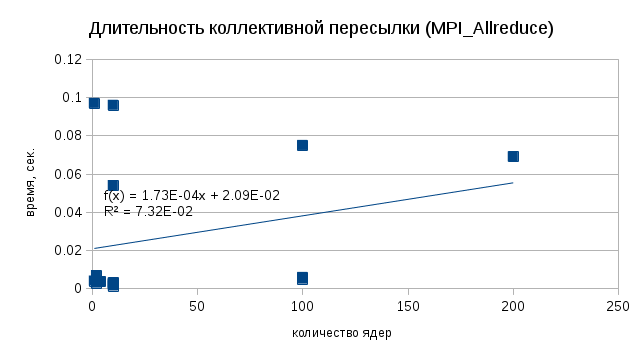
\includegraphics[height=7cm,keepaspectratio]{images/RomanenkoAASnytnikovAVChernykhIGadaptationtosupercomputerfinalEXTENDEDREFERENCES-img2.png}
        	\end{center}
        	\caption{Продолжительность операции MPI\_Allreduce. Линейная аппроксимация.}
        	\label{lin_appr}
        \end{figure}
        
        %Рис.2. Продолжительность операции MPI\_Allreduce. Линейная аппроксимация.
        
        \begin{figure}[htb]
        	\begin{center}
        		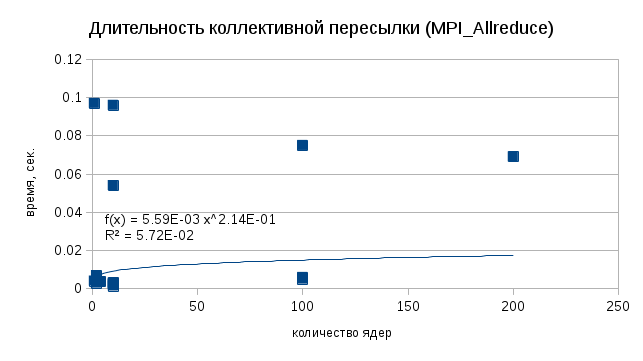
\includegraphics[height=7cm,keepaspectratio]{images/RomanenkoAASnytnikovAVChernykhIGadaptationtosupercomputerfinalEXTENDEDREFERENCES-img3.png}
        	\end{center}
        	\caption{Продолжительность операции MPI\_Allreduce. Степенная аппроксимация.}
        	\label{power_appr}
        \end{figure}
        
      %  Рис.3. Продолжительность операции MPI\_Allreduce. Степенная аппроксимация.
       
       
       \begin{figure}[htb]
       	\begin{center}
       		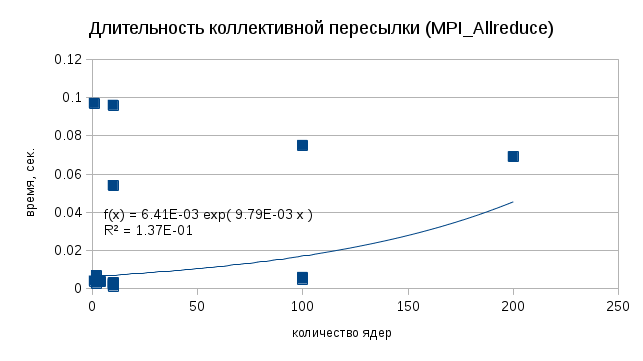
\includegraphics[height=7cm,keepaspectratio]{images/RomanenkoAASnytnikovAVChernykhIGadaptationtosupercomputerfinalEXTENDEDREFERENCES-img4.png}
       	\end{center}
       	\caption{Продолжительность операции MPI\_Allreduce. Экспоненциальная аппроксимация.}
       	\label{exp_appr}
       \end{figure} 
       % Рис.4. Продолжительность операции MPI\_Allreduce. Экспоненциальная аппроксимация.
        Из рисунков \ref{lin_appr,power_appr,exp_appr} видно, что наименьшее значение среднеквадратической ошибки достигнуто при степенной аппроксимации:
        $$
        T = 0.0056*N^{0.214}
        $$
        \clearpage
        
        Далее рассмотрим парные пересылки. Зависимость от числа ядер в данном случае возникает потому, что в таких пересылках задействованы все ядра, между которыми разделена область: MPI-процесс, работающий на каждом ядре пересылает данные обоим своим соседям. Фактически речь идет о длительности эйлерова этапа параллельного алгоритма.
        
         \begin{figure}[htb]
         	\begin{center}
         		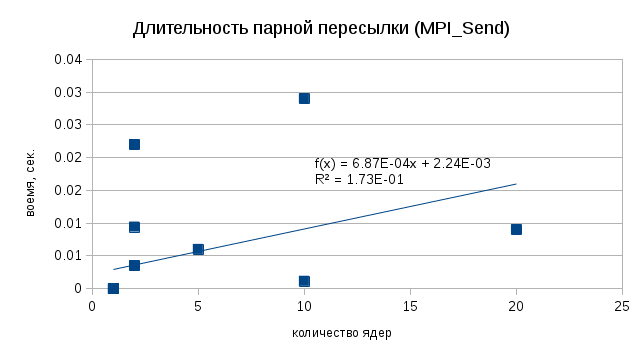
\includegraphics[height=7cm,keepaspectratio]{images/RomanenkoAASnytnikovAVChernykhIGadaptationtosupercomputerfinalEXTENDEDREFERENCES-img5.png}
         	\end{center}
         	\caption{Продолжительность операции MPI\_Send. Линейная аппроксимация.}
         	\label{send_lin_appr}
         \end{figure}
         
         %Рис.2. Продолжительность операции MPI\_Allreduce. Линейная аппроксимация.
         
         \begin{figure}[htb]
         	\begin{center}
         		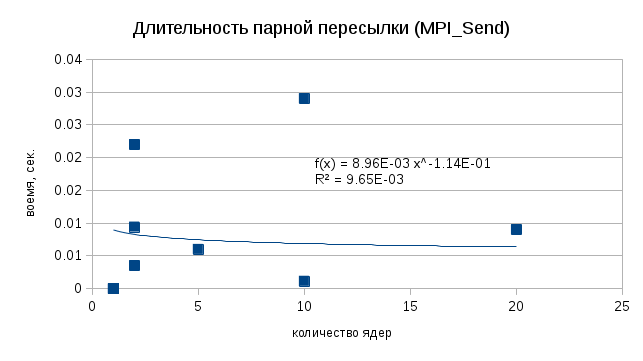
\includegraphics[height=7cm,keepaspectratio]{images/RomanenkoAASnytnikovAVChernykhIGadaptationtosupercomputerfinalEXTENDEDREFERENCES-img6.png}
         	\end{center}
         	\caption{ Продолжительность операции MPI\_Send. Степенная аппроксимация.}
         	\label{send_power_appr}
         \end{figure}
         
         %  Рис.3. Продолжительность операции MPI\_Allreduce. Степенная аппроксимация.
         
         
         \begin{figure}[htb]
         	\begin{center}
         		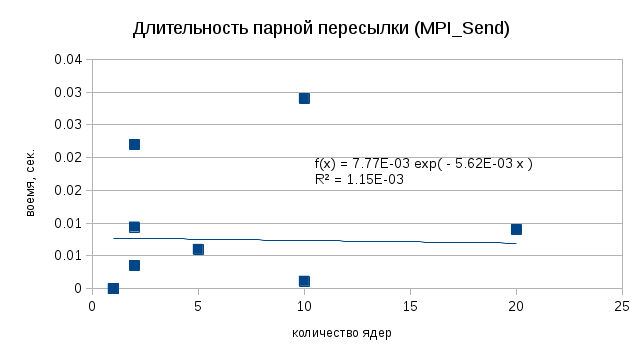
\includegraphics[height=7cm,keepaspectratio]{images/RomanenkoAASnytnikovAVChernykhIGadaptationtosupercomputerfinalEXTENDEDREFERENCES-img7.png}
         	\end{center}
         	\caption{Продолжительность операции MPI\_Send. Экспоненциальная аппроксимация.}
         	\label{send_exp_appr}
         \end{figure} 
         
        В этом случае наименьшая ошибка оказалась достигнута при экспоненциальной аппроксимации:
        
        $$
        T = 0.0077*exp(-0.00562*N)
        $$
        
        
        Полученные формулы не является зависимостями, работающими всегда, на любых суперЭВМ, любых реализациях MPI и т.д. Их назначение в том, чтобы в ходе реального крупномасштабного расчета, без повторных запусков, не прерывая счет, ответить на вопрос, что будет, если увеличить количество процессоров (ядер), вовлеченных в коллективные взаимодействия. Т.е. в данном случае предполагается динамическое дозапускание MPI процессов, допустимое стандартом MPI2.
        Например, программа, использующая 40 MPI-процессов  получила для счета 40 ядер. Эти ядра можно по-разному распределить между эйлерой и лагранжевой декомпозицией области: можно поделить область на 10 частей, и затем распределить все частицы каждой подобласти между  4 MPI-процессами, а можно наоборот. Даже для 40 процессов есть несколько вариантов, в то время как речь идет о расчетах на нескольких тысячах ядер, где невозможно будет просто перебрать все варианты и выбрать оптимальный.
        Для того, чтобы сделать правильный выбор, предлагается после выделения узлов для счета провести несколько тестовых запусков коллективных операций, построить для данного конкретного расчета аппроксимацию, подобную полученной выше, и на ее основе принимать решение.
        
        
        \section{Обеспечение возможности эффективного использования сверхбольших ВС на основе тестирования с помощью метода частиц в ячейках}
        
        Вначале необходимо ответить на вопрос о принципиальной возможности решения указанной выше задачи, или о наличии оборудования, позволяющего проводить расчеты настолько большой размерности. Поставленная задача (об обеспечении возможности расчета на сетке в 1 трлн. узлов) должна решаться в несколько этапов, во-первых, потому что категорически неправильно начинать расчеты сразу с модели большого размера, во вторых потому что для проведения расчета с указанными выше параметрами необходимо около 800 тыс. процессоров, если исходить из параметров вычислительных узлов основного раздела суперкомпьютера «Ломоносов» (по состоянию на июнь 2016 года).
        
        Вначале будет рассматриватьcя несколько промежуточных задач начиная от размерности в 10 млн. узлов, которая эффективно решается в настоящий момент на кластере небольшого размера, далее в 1 млрд. узлов, эффективное решение которой с учетом модельных частиц потребует использование до 1000 процессоров. Следующая сетка будет иметь размер 10 млрд. узлов, для решения такой задачи потребуется примерно вдвое больше процессоров, чем содержится в основном разделе суперкомпьютера «Ломоносов». Для этих задач меньшего размера должна быть продемонстрирована высокая эффективность распараллеливания, в том числе до нескольких тысяч процессоров. Это даст возможность подавать мотивированную заявку на большее количество вычислительных ресурсов, например, на монопольное использование суперкомпьютера «Ломоносов» (это потребуется уже для сетки в 100 млрд. узлов), или на зарубежные суперЭВМ.
        
        Как было отмечено в разделе «цели и задачи фундаментального исследования», метод частиц используется в данной задаче в силу того, что он дает наиболее точное приближение вида функции распределения частиц. Альтернативой методу частиц является прямой метод решения уравнения Власова, но такой вариант потребует значительно больших затрат по памяти. Говоря о степени новизны такого подхода, важно заметить, что в основном в мировой практике для решения задач физики ускорителей в основном используются более упрощенные модели, например, модель листов (D. Schulte. TESLA-97-08 (1996)). Модели на основе метода частиц являются более точными, но и значительно более трудоемкими. Таким образом, использование больших мощностей суперЭВМ позволяет внести существенный элемент новизны в моделирование динамики встречных пучков (М.А.Боронина, канд.дисс.).
        
        Целью проекта является создание и программная реализация параллельного алгоритма, способного обеспечить эффективность распараллеливания в слабом смысле выше 90 % до нескольких сотен тысяч процессоров. Такую высокую эффективность предлагается достигать за счет реализации схемы трехмерной эйлерово-лагранжевой декомпозиции расчетной области с использованием централизованного алгоритма динамической балансировки загрузки.
        
        Под эйлерово-лагранжевой декомпозицией имеется в виду следующее: расчетная область разделяется на подобласти (сетка вместе с частицами), и затем, при необходимости, частицы отдельной подобласти дополнительно разделяются между процессорами. Эйлеро-лагранжева декомпозиция предложена А.В.Снытниковым в 2009 (труды конференции “Научный сервис в сети Интернет-2009”). Аналогичная концепция под названием виртуальных слоев реализована М.А.Краевой и В.Э.Малышкиным (Malyshkin, Kraeva, FGCS, 2001), а также C.Othmer (Othmer, CPC, 2002) под названием “ферма задач” (taskfarm). Существенный элемент новизны, тем не менее, заключается, во-первых, к примению к области физики ускорителей, и таким образом к решению задач очень большого объема и во-втрорых, в том, что в обоих описанных выше случаях описаны инструменты для устранения локальной несбалансированности загрузки, а предлагамом проекте предполагается созданием алгоритма с глобально в целом однородной загруженностью. Основным результатом использования эйлерово-лагранжевой декомпозиции будет снижение количества межпроцессорных комуникаций. Масштабируемость варианта эйлерово-лагранжевой декомпозиции расчетной области подтверждается теоретическими соображениями, высказанными в работах В.Э.Малышкина (V.E.Malyshkin, PaCT-99 proceedings), а именно сведением размера минимального фрагмента фактически к размеру одной частицы и выполнением условия линейности алгоритма.
        
        Также для эффективной реализации метода частиц в ячейках на будет использована технология решения задач физики плазмы на суперЭВМ (А.В.Снытников, доклады конференции «Супервычисления и математическое моделирование», г.Саров 2016). Очевидно, что между задачами физики плазмы и физики ускорителей существуют фундаментальные различия. Вместе с тем общность основных используемых уравнений позволяет использовать методы и подходы, отработанные при решении плазменных задач, для задач физики ускорителей. Основными элементами технологии являются, кроме эйлерово-лагранжевой декомпозиции расчетной области, реализация наиболее трудоемких расчетных процедур на ускорителях вычислений, параметризованная форма реализации метода частиц в ячейках для быстрой замены численных методов, и методика межархитектурного переноса программ, для того, чтобы не зависеть от конкретной архитектуры суперЭВМ. Предлагаемая технология в целом является новой, несмотря на то, что ее отдельные элементы имеют пересечения с зарубежными работами (Vazquez
        et al.,J.Comp.Sci, 2016, Decyk, Comp.Phys.Comm., 2011).
        
        Предполагается создание централизованного алогоритма балансировки. Сама по себе идея не явяется новой, она описана в большой количестве работ, например Wolfheimer, 2006 или A.Vinay, 2011. Элементом новизны является учет особенностей решаемой задачи о динамике частиц в ускорителе. При этом движение частиц может иметь характер быстрых осцилляций, так что частица проходит незначительно расстояние, но очень большое количество ячеек сетки. Сущность предлагаемого алгоритма балансировки загрузки заключается в том, чтобы выявлять на основе физических параметров области с потенциально возможным множественным перемещением частиц, и менять декомпозицию таким образом, чтобы все этой движение происходило в рамках одной параллельной подобласти, т.е. без пересылок частиц между процессорами, при этом вычислением движения частиц в этой подобласти могут быть заняты несколько процессоров. Осуществить это можно, например, перемещая подобласть вслед за пучком.
        
        Основная особенность параллельного алгоритма, который будет создан в ходе выполнения проекта – использование динамического варианта декомпозиции. Это означает, что первоначально запускается, например, чисто лагранжева декомпозиция, далее, если в процессе работы по результатам измерения производительности как вычислительного алгоритма, так и пересылок, становится видно, что используемый вариант неэффективен, то происходит переход к одномерной эйлеровой декомпозиции, или двух-, трехмерной если
        потребуется, и в итоге, к заявленной трехмерной эйлерово-лагранжевой декомпозиции.
        
        Методы прогнозирования эффективности работы параллельного алгоритма на основе имеющихся данных об архитектуре и производительности отдельных элементов суперЭВМ будут созданы на основе оценочных формул, известных, в частности по работам С.А.Степаненко \cite{StepanenkoScaling} и И.Н. Молчанова («Введение в алгоритмы параллельных вычислений», 1990), а также методов иммитационного моделирования (D. Podkorytov, A. Rodionov, H. Choo,Proceedings of the 6th International Conference on Ubiquitous Information Management and Communication ACM, 2012). Новизна в данном случае заключается во встройке методов прогнозирования непосредственно в вычислительный алгоритм с тем, чтобы эффективность работы алгоритма была не результатом работы программы, а изначальным требованием, которому программа так или иначе должна сооотвествовать.
        
        Расчеты с использованием большого количества процессоров предполагается проводить на суперЭВМ “Ломоносов” и “Ломоносов-2”, а также на кластере СпбГТУ “Политехник”, при достижении высокой эффективности для маскимально доступного на этих суперЭВМ числа процессоров предполагается подать заявку на использование ресурсов европейского сообщества супервычислений PRACE.
        
        
        \section{Опредедение зависимости масштабируемости от наличия и типа ускорителей вычислений}
        
        \textbf{Масштабируемость для кластера на основе Intel Xeon Phi.} 
        
       Также было проведено тестирование масштабируемости программы на кластере RSC Petastream в МСЦ РАН, результат показан на рис. \ref{phi100}. Видно, что в целом программа хорошо масштабируется, локальный максимум, видимый на графике при 5 ускорителях, может объясняться тем, что система на тот момент работала в тестовом режиме.
        
        \begin{figure}[htb]
        	\begin{center}
        		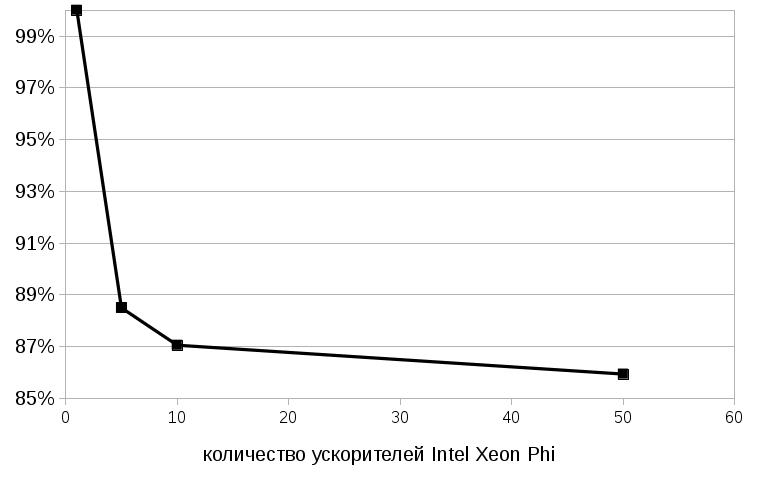
\includegraphics[height=7cm,keepaspectratio]{images/petastream_phi100.jpg}
        	\end{center}
        	\caption{Эффективность распараллеливания в слабом смысле с использованием Intel Xeon Phi. Расчет проведен на суперкомпьютере RSC Petastream, МСЦ РАН.}
        	\label{phi100}
        \end{figure}
        
        Также было выполнено распалаллеливание на мелкозернистом уровне: по отдельным частицам в рамках ячейки: отдельные вычислительные потоки назначаются для счета траекторий отдельных частиц. Это было выполнено с помощью технологии CUDA для графических ускорителей (GPU) и с помощью технологии OpenMP для ускорителей Intel Xeon Phi. Программа MANAS может быть скомпилирована как для одного типа ускорителей (GPU). Так и для другого (Intel Xeon Phi). Это достигается с помощью процедурных переменных и директив условной компиляции. Программа протестирована на кластере НКС-30Т (ИВМиМГ СО РАН), графические ускорители Nvidia Tesla M2090 (до 10) и Nvidia Kepler K40 и на суперЭВМ «Ломоносов»  (до 500 Nvidia Tesla C2070). Средняя продолжительность одного временного шага 0.01 секунды для  Nvidia Kepler K40 и 0.13 секунды для  Intel Xeon Phi (сетка 250х250, 100 частиц).
        
        \begin{figure}[htb]
        	\begin{center}
        		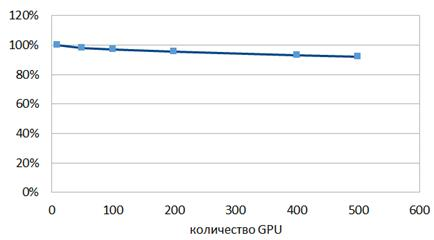
\includegraphics[height=7cm,keepaspectratio]{images/lomonosov_gpu500.jpg}
        	\end{center}
        	\caption{Эффективность распараллеливания в слабом смысле. Расчет проведен на суперкомпьютере «Ломоносов», НИВЦ МГУ.}
        	\label{gpu500}
        \end{figure}
        
        Из сравнения рисунков \ref{phi100} и \ref{gpu500} видно, что наличие ускорителей вычислений не дает каких-то особенностей в работе коммуникационной системы ВС, и таким образом, коммуникационная система может анализироваться независимо от типа узлов ВС.
          
        
        
        
        
        
        
        \section{Определение коммуникационной структуры ВС}
        
        MPI предоставляет пользователю возможность создания собственных виртуальных топологий, в том числе декартовых (двумерных, трехмерных  и пр.). При этом в соответствии со стандартом процессы, расположенные на физически близких узлах, должны иметь близкие номера в рамках топологии, однако все зависит от конкретной реализации MPI.  
        
        Для решения этого вопроса в описанной программе реализован специальный диагностический модуль, выполняющий пересылки типа «точка-точка» (MPI\_Send/MPI\_Recv) между всеми процессами (all-to-all, «каждый с каждым»). При этом рассматривались разные варианты размещения процессов по узлам. В каждом случае измерялось время пересылки с помощью функции MPI\_Wtime. На рисунках 8-13 показано время пересылок во всех парах взаимодействующих процессов.
        
        \begin{figure}[htb]
        	\begin{center}
        		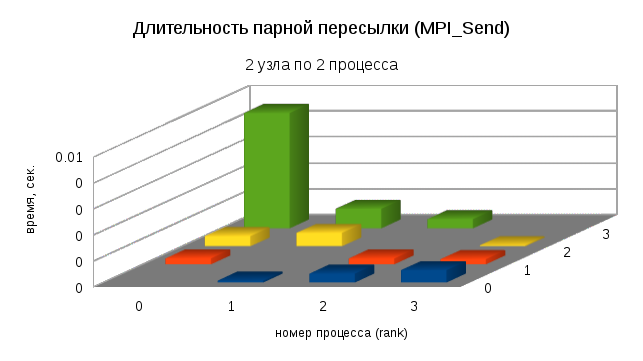
\includegraphics[height=7cm,keepaspectratio]{images/RomanenkoAASnytnikovAVChernykhIGadaptationtosupercomputerfinalEXTENDEDREFERENCES-img8.png}
        	\end{center}
        	\caption{ Время пересылок для 4 MPI-процессов, расположенных на двух узлах попарно, кластер НГУ.}
        	\label{2nodeNSU}
        \end{figure}
        
        
        На рисунке \ref{2nodeNSU} видно, что время пересылок внутри узла (0-й процесс и 1-й, или 3-й и 4-й) меньше, чем время пересылок между узлами. Для того, чтобы аналогичным образом рассмотреть более сложные конфигурации, необходимо перейти от трехмерной столбчатой диаграммы к двумерным картам плотности, например, рис.\ref{NSU16}. 
        
        \begin{figure}[htb]
        	\begin{center}
        		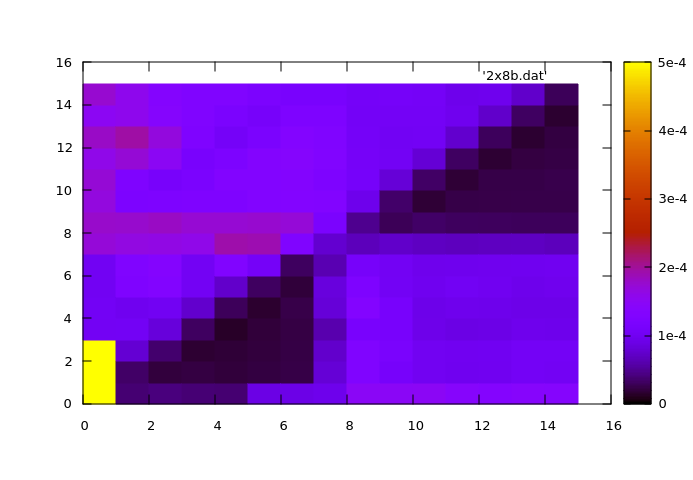
\includegraphics[height=7cm,keepaspectratio]{images/RomanenkoAASnytnikovAVChernykhIGadaptationtosupercomputerfinalEXTENDEDREFERENCES-img9.png}
        	\end{center}
        	\caption{ Время пересылок для 16 MPI-процессов, расположенных на двух узлах по 8 процессов, кластер НГУ. По осям X и Y отложены номера процессов, цветовая шкала показывает время пересылок в секундах.}
        	\label{NSU16}
        \end{figure}
        
        
        Рисунок \ref{NSU16} естественным образом разбивается на 4 зоны, соответствующих размещению процессов по узлам, несмотря на то, что принципиальной разницы по времени пересылок между узлами и внутри узлов в данном случае нет.
        
        \begin{figure}[htb]
        	\begin{center}
        		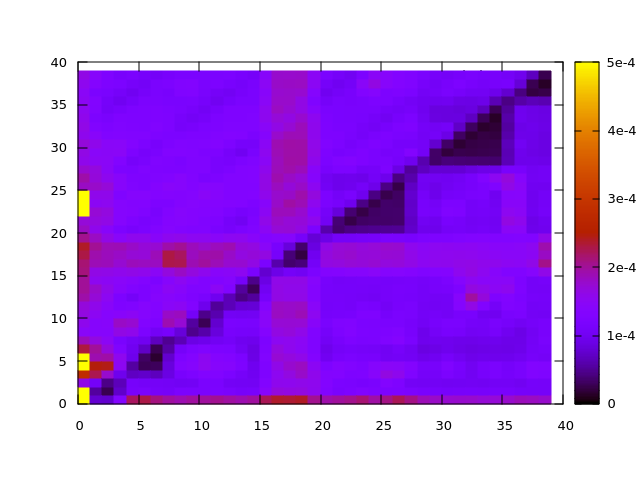
\includegraphics[height=7cm,keepaspectratio]{images/RomanenkoAASnytnikovAVChernykhIGadaptationtosupercomputerfinalEXTENDEDREFERENCES-img10.png}
        	\end{center}
        	\caption{ Время пересылок для 40 MPI-процессов, расположенных на 10 узлах по 4 процесса, кластер НГУ. По осям X и Y отложены номера процессов, цветовая шкала показывает время пересылок в секундах.}
        	\label{NSU40}
        \end{figure}
        
       
        На рисунке \ref{NSU40} не удается зрительно выделить 10 зон, соответствующих 10 узлам, на которые проводился расчет. Тем не менее видно, что участки с наименьшими временами пересылок расположены вдоль диагонали матрицы, как и на предыдущих рисунках.
        Следует отметить, что такая задача безусловно и не должна решаться «на глаз», в дальнейшем планируется применить здесь известные методы выделения сообществ в полном графе. Задача данной работы только в том, чтобы проверить обмен сообщениями у попарно между всеми процессами как метод тестирования архитектуры кластера: позволяет ли он выявлять отличие между близко и далеко расположенными процессами. Для этого обратимся к ВС существенно отличной архитектуры, а именно кластеру «Политехник» в СПбПУ.
        
        \begin{figure}[htb]
        	\begin{center}
        		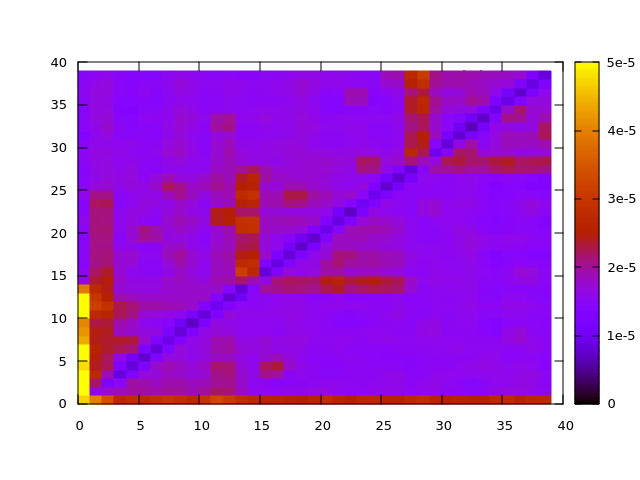
\includegraphics[height=7cm,keepaspectratio]{images/RomanenkoAASnytnikovAVChernykhIGadaptationtosupercomputerfinalEXTENDEDREFERENCES-img11.png}
        	\end{center}
        	\caption{Время пересылок для 40 MPI-процессов, расположенных на 10 узлах по 4 процесса, кластер «Политехник», СПбПУ. По осям X и Y отложены номера процессов, цветовая шкала показывает время пересылок в секундах.}
        	\label{Poly40}
        \end{figure}
        
        
       
        В первую очередь важно отметить, что на рисунке \ref{Poly40} все времена на порядок меньше, чем на рис.\ref{NSU40} , показывающем ту же конфигурацию для кластера НГУ. Далее, на рис.\ref{Poly40} видны прямоугольные участки с большим временем пересылок (красного цвета), шириной в 4 процесса, расположенные как горизонтально, так и вертикально. Это говорит о том, что возможна ситуация, когда близко по номеру расположенные процессы будут иметь большее время обмена сообщениями по сравнению с более удаленными (в данном случае 13-15 процессы при обмене с  16-20 процессами). 
        
         \begin{figure}[htb]
         	\begin{center}
         		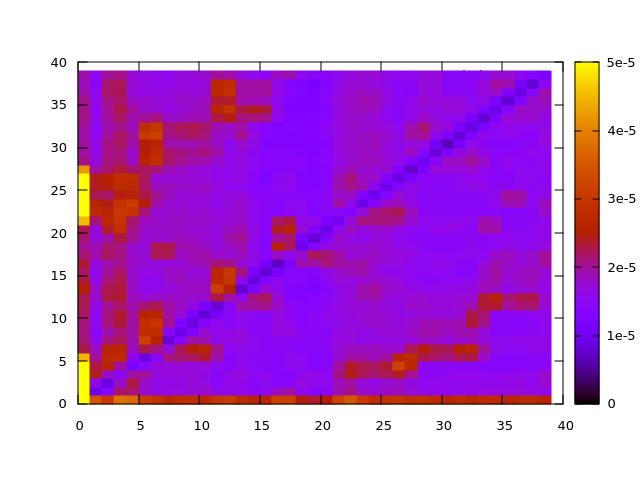
\includegraphics[height=7cm,keepaspectratio]{images/RomanenkoAASnytnikovAVChernykhIGadaptationtosupercomputerfinalEXTENDEDREFERENCES-img12.png}
         	\end{center}
         	\caption{Время пересылок для 40 MPI-процессов, расположенных на 4 узлах по 10 процессов, кластер «Политехник», СПбПУ. По осям X и Y отложены номера процессов, цветовая шкала показывает время пересылок в секундах.}
         	\label{Poly4_10}
         \end{figure}
        
        
        На рис. \ref{Poly4_10} показан расчет также с использованием 40 процессов, но размещенных на 4 узлах. Видно, что красные зоны (с большим временем пересылок) имеют больший размер и преимущественно локализованы в левой верхней и правой нижней четвертях квадрата, что соответствует обмену сообщениями между процессами, расположенными на разных узлах.
        
         \begin{figure}[htb]
         	\begin{center}
         		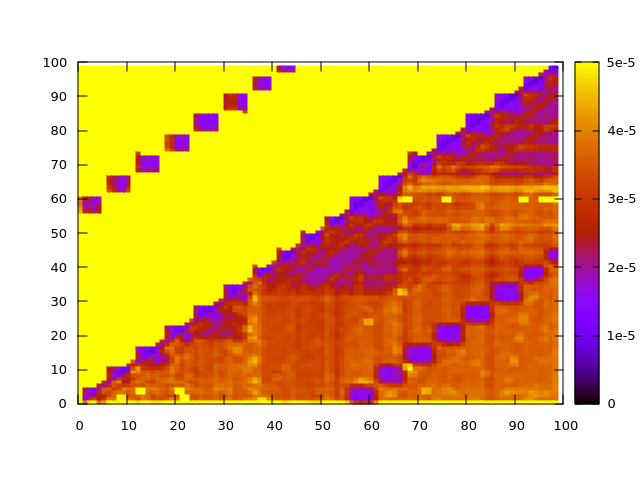
\includegraphics[height=7cm,keepaspectratio]{images/RomanenkoAASnytnikovAVChernykhIGadaptationtosupercomputerfinalEXTENDEDREFERENCES-img13.png}
         	\end{center}
         	\caption{Время пересылок для 100 MPI-процессов, расположенных на 10 узлах по 10 процессов, кластер «Политехник», СПбПУ. По осям X и Y отложены номера процессов, цветовая шкала показывает время пересылок в секундах.}
         	\label{Poly10_10}
         \end{figure}
        
       
        На рисунке \ref{Poly10_10} видны группы размером 5 процессов, время обмена между которыми заметно меньше, чем со всеми остальными. Это также коррелирует с их размещением по узлам.
        
        
        
   \clearpage     
        
        
        
       
        
        
		\subsubsection{Измерение производительности коммуникационной сети на основе данных о пересылке модельных частиц}
		В \textit{четвертом разделе} приведены результаты измерения скорости пересылок модельных частиц в методе частиц в ячейках и проведенный на основе этого сравнительный анализ скорости работы коммуникационной сети ВС.
		
		На нескольких параллельных ВС были измерены времена, затраченные на пересылку модельных частиц между соседними узлами. Из статитики расчетов по методу частиц в ячейках известно, что пересылается, как правило, не более 5\% модельных частиц. В рассматриваемых расчетах размер сетки $512\times 64 \times 64$ узла  при 150 модельных частицах в ячейке, т.е.  на каждом временном шаге в среднем пересылается 15.7 млн. модельных частиц, что при размере одной частицы в 48 байт означает 720 Мб на каждый временной шаг, что при известном времени пересылки позволяет вычислить скорость. Таким образом была экспериментально измерена величина $T_{P,S}$, входящая в формулу \ref{PIC-timestep}   
			
			
			
			Измеренная таким образом скорость пересылки данных показывает фактический предел этой величины, реально достижимый для вычислительного приложения с использованием имеющегося оборудования и коммуникационного программного обеспечения. Это подтверждается следующими соображениями:
			\begin{itemize}
				\item Объем пересылаемых данных мал: в среднем 6 Мб на процесс
				\item Соседние MPI-процессы, как правило, расположены на близких узлах.
			\end{itemize}  	 
			
		%	\subsubsection{Экстраполяция результатов тестирования ускорения и эффективности распараллеливания}
			%%	формулы из статьи НГУ-ИТ'17, адаптированные и улучшенные, сравнение со Степаненко
			%%	выводы по большой системе на тех же принципах, совпадение с реальностью
			%%	
			%	В \textit{четвертом разделе} описана оригинальная методика экстраполяции результатов на системы большой размерности и ее сравнение с аналогиными работами.Проведено большое количество физических расчетов с использованием программы в трехмерной расчетной области, использующей двухступенчатую эйлерово-лагранжеву декомпозицию расчетной области.На основании тестовых расчетов на небольшом количестве процессорных ядер измереятся время коллективных и парных коммуникаций MPI и строится аппроксимацию времени пересылок для произвольного количества процессов.
			
			%	Основным вопросом является соответствие реально измеряемого времени выполнения коммуникационных операций для определенного количества процессоров, 
			%	 По результатам вырабатываются рекомендации по выбору оптимального сочетания эйлеровой и лагранжевой декомпозиции.
			%	\textbf{формулы}
			
			%	\subsection{Глава 3: Анализ производительности системы памяти}
			%	\subsubsection{Кэш-память}    
			%	Статьи PACO (кэш, списки и пр.), BOE (данны исполения на Sun Sparc Opteron)
			%	\subsubsection{Оперативная память}
			%	 PAVT10, Абрау7 PACO